\section{Aprendizaje Maquina}
\label{sec:MachineLearning}

La inteligencia artificial incorpora un conjunto diverso de trabajos relacionados con el razonamiento automático mientras que el subcampo del aprendizaje maquina se especializa en el reconocimiento de patrones y el aprendizaje de los datos (\cite{rosebrock2017deep}).

El aprendizaje maquina utiliza algoritmos para extraer información o patrones de un conjunto de datos(\textit{Dataset}) sin procesar y representarla en un modelo, después usar este modelo para inferir resultados sobre otros datos que aún no hemos modelado (\cite{patterson2017deep}).

El aprendizaje maquina utiliza estadísticas.Tradicionalmente se resuelve un problema determinista en el que nuestra solución resuelve el problema todo el tiempo. Hay muchos problemas en los que la solución no es determinista. Es decir, no sabemos lo suficiente sobre el problema o no tenemos suficiente potencia para modelar correctamente el problema. Para estos problemas necesitamos estadísticas(\cite{harrington2012Machine}).

En otras palabras, el aprendizaje maquina es un subcampo de la inteligencia artificial, este se encarga de aprender los patrones con los cuales podemos modelar un conjunto de datos, una vez aprendido los patrones más importantes se crea un modelo que podemos utilizar para identificar cierto conjunto de datos.

La metodología utilizada en el aprendizaje maquina es relativamente sencilla, por ejemplo, si queremos aprender a identificar si una imagen contiene un animal como un ratón o un gato, debemos tomar cierto número de muestras(cientos o miles). Con estas muestras el aprendizaje maquina se encargará de tomarlas y procesarlas para identificar las caracterizas más importantes, estas características son el modelo que define a cada animal. Ahora bien, podemos tomar una de las muestras y pasarla por el modelo creado, con esto es muy probable que el modelo nos diga correctamente que animal esta la imagen, es por esto que se utilizan muestras que no hayan sido procesadas anteriormente.

La RAE define aprender como adquirir el conocimiento de algo por medio del estudio o de la experiencia, en nuestro caso la maquina aprende por medio de la experiencia adquirida al procesar cada una de las muestras, a tal grado que identifica muestras que no estaban en el conjunto de datos de entrada. En aprendizaje maquina se le llama entrenamiento al proceso de generación de un modelo a partir de las muestras, mientras que la validación es el proceso con el cual el modelo infiere resultados a partir de muestras que no pasaron por el proceso de entrenamiento. El conjunto de datos son todas las muestras que serán utilizadas para el proceso de entrenamiento y validación.

Comúnmente el conjunto de datos es dividido para cada proceso, entrenamiento y validación, en la práctica lo más común es separar el conjunto de un porcentaje de 70-30, siendo 70\% para el proceso de entrenamiento y 30\% para la validación.

Mas adelante se presentan las métricas que se utilizan para evaluar el modelo por medio del conjunto de datos de validación. En el aprendizaje maquina tenemos tres tipos diferentes de aprendizaje: aprendizaje supervisado, aprendizaje no supervisado y aprendizaje semi-supervisado, a continuación, se describen los tres tipos de aprendizaje, sin embargo, en este trabajo solo se hablará con más detalle sobre el aprendizaje supervisado.

\begin{itemize}

    \item Aprendizaje supervisado: Es un proceso de entrenamiento en el que se realizan predicciones sobre los datos de entrada y luego se corrigen las predicciones incorrectas. El proceso continúa hasta que se obtiene un error bajo o un número máximo de iteraciones. Para esto es necesario que nuestros datos de entrada tengan cierta etiqueta con el significado de cada uno de nuestros datos.

    \item Aprendizaje no supervisado: En este aprendizaje no tenemos nuestros datos con la etiqueta correspondiente a su valor. Para este caso es el entrenamiento el encargado de encontrar cierto patrón en los datos con el cual asignara una etiqueta a cada uno de ellos.

    \item Aprendizaje semi-supervisado: En el aprendizaje semi-supervisado tenemos datos etiquetados y datos sin etiquetar. El proceso de entrenamiento toma los datos conocidos, los analiza y etiqueta cada uno de los datos no etiquetados para usarlos como datos de entrenamiento adicionales. El algoritmo semi-supervisado aprende la “estructura" de los datos.

\end{itemize}


\subsection{Aprendizaje supervisado}

En la Sección \ref{sec:MachineLearning} menciono un poco sobre el aprendizaje supervisado, ahora vamos a hablar sobre dos tipos de problemas que nos podemos encontrar al resolverlos utilizando aprendizaje máquina.

\subsubsection{Clasificación}

En el aprendizaje maquina la clasificación consiste en que el algoritmo aprenda los patrones que definen un conjunto de datos perteneciente a una clase especifica. Los valores de salida del modelo es la categoría correspondiente a los datos de entrada que pueden ser dos o más opciones bien definidas.

La clasificación binaria es la forma más simple de clasificación en esta se tienen solo dos valores de salida (0 o 1). Esta clasificación nos sirve para responder a la simple pregunta si pertenece o no a una clase en concreto. Por ejemplo, podemos identificar si una transacción bancaria es fraudulenta o no.

Existen una gran variedad de conjuntos de datos con una gran cantidad de clases como MNIST, Animals, CIFAR-10, Flowers-17 entre otros cada uno de estos son útiles para validar el correcto funcionamiento de una red neuronal.

\begin{figure}[H]
    \centering
    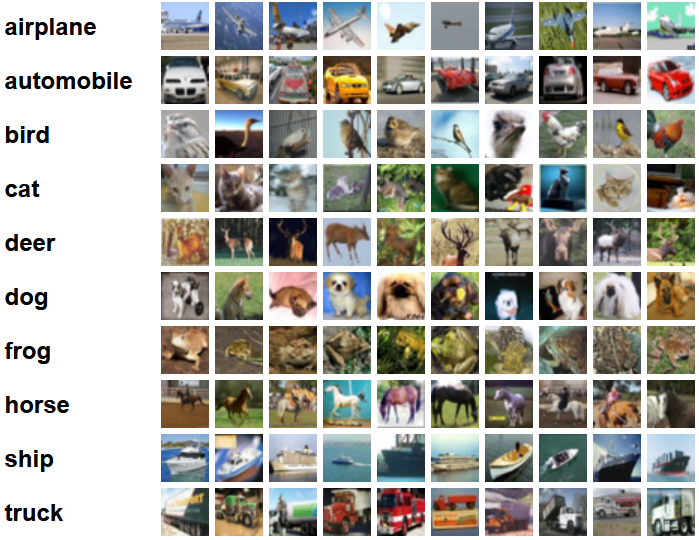
\includegraphics[width=0.6\textwidth]{MarcoTeorico/imgs/CIFAR-10.png}
    \caption{\textit{Dataset} CIFAR-10.}
    \label{fig:cifar10}
\end{figure}

Para todo aquel problema que implique separar un conjunto de datos en diferentes clases o categorías, sin importar el numero clases que pueden ser, se utiliza la clasificación.

\subsubsection{Regresión}

Los problemas de regresión predicen un valor real. En otras palabras, la función que estima la variable dependiente conociendo la variable independiente.

La regresión es utilizada para aquellos problemas que implican predecir valores numéricos, un ejemplo de esto son las predicciones de ráfagas de vientos las cuales dando como entrada diferentes características del ambiente podemos predecir la velocidad del viento.

\subsubsection{Regresión Lineal}

La clase más común de regresión es la regresión lineal. La regresión lineal intenta llegar a una función que describa la relación entre $x$ y $y$, para valores conocidos de $x$, predice valores de $y$ que resultan ser precisos (\cite{patterson2017deep}). La Figura \ref{fig:regresionLineal} representa la regresión en una gráfica.

\begin{figure}[H]
    \centering
    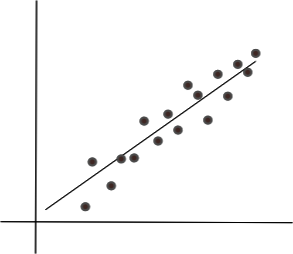
\includegraphics[width=0.5\textwidth]{MarcoTeorico/imgs/RegresionLineal.png}
    \caption{Grafica de regresión lineal.}
    \label{fig:regresionLineal}
\end{figure}

\subsubsection{Regresión Ridge}

La regresión Ridge es una versión regularizada de la regresión lineal, agrega un término de regularización en la función de costo (Ecuación \ref{eq:ridge}). Con esto se busca que el algoritmo mantenga los pesos lo más pequeños posible.

\begin{equation}
    \label{eq:ridge}
    \alpha \displaystyle\sum\limits_{i=1}^n (\theta_i)^{2}
\end{equation}

El hiperparametro $\alpha$ controla la regularización del modelo, si $\alpha = 0$ la regresión Ridge es simplemente una regresión lineal. Si $\alpha$ es muy grande, todos los pesos terminan igual a cero y resulta en una línea plana que pasa por la media de los datos(Figura \ref{fig:regresionRidge}.

\begin{figure}[H]
    \centering
    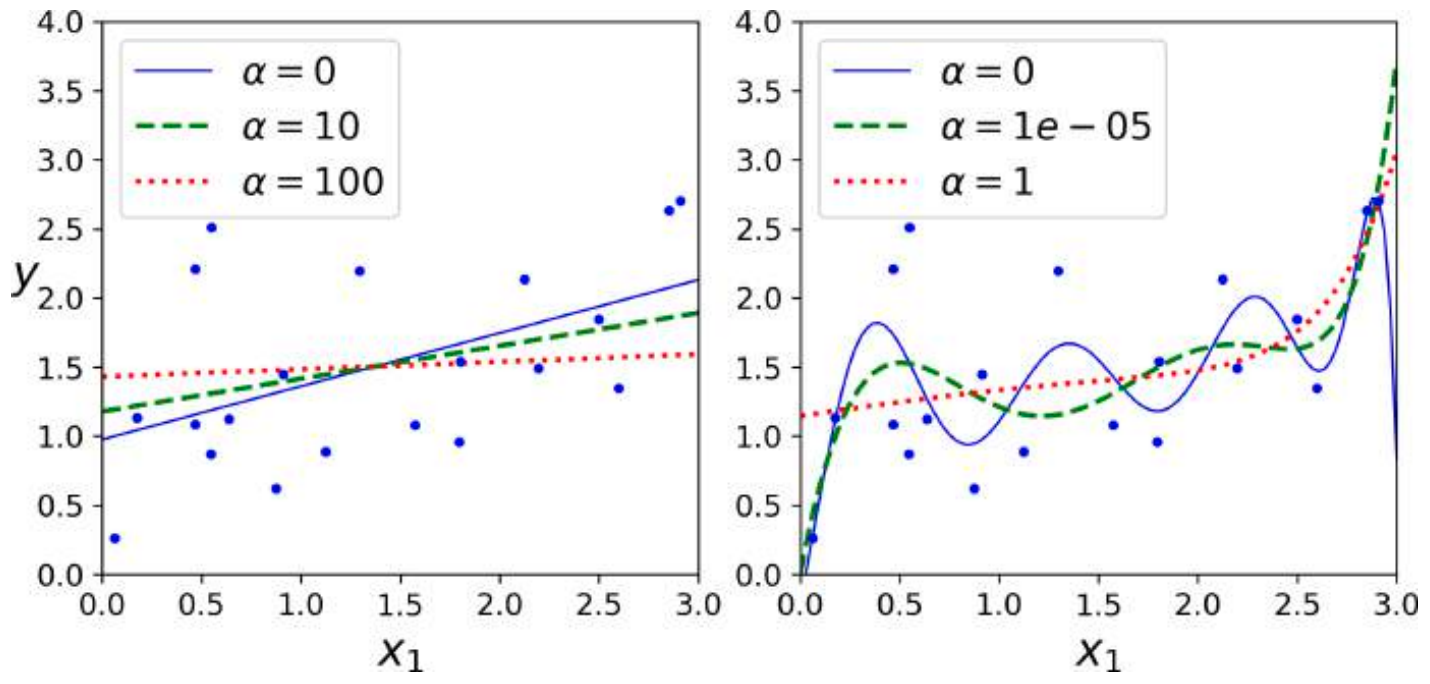
\includegraphics[width=0.8\textwidth]{MarcoTeorico/imgs/Ridge.png}
    \caption{Regresión Ridge con diferentes valores de $\alpha$.}
    \label{fig:regresionRidge}
\end{figure}

La Ecuación \ref{eq:ridgeCostFunction} es la función de costo para la regresión Ridge.

\begin{equation}
    \label{eq:ridgeCostFunction}
    J(\theta) = MSE(\theta)
    + \alpha \displaystyle\sum\limits_{i=1}^n (\theta_i)^{2}
\end{equation}

\subsubsection{Regresión Lasso}

La regresión Lasso (\textit{Least Absolute Shrinkage and Selection Operator} en Ingles) al igual que la regresión Ridge es una versión regularizada de la regresión lineal, sin embargo, la regresión Lasso utilizada valores absolutos en la función de regulación (Ecuación \ref{eq:lasso}), una característica importante con Lasso es que puede llegar a eliminar por completo los pesos de las características menos importantes.

\begin{equation}
    \label{eq:lasso}
    \alpha \displaystyle\sum\limits_{i=1}^n  \mid \theta_i \mid
\end{equation}

La Ecuación \ref{eq:lassoCostFunction} es la función de costo para la regresión Lasso.

\begin{equation}
    \label{eq:lassoCostFunction}
    J(\theta) = MSE(\theta)
    + \alpha \displaystyle\sum\limits_{i=1}^n  \mid \theta_i \mid
\end{equation}

\subsubsection{Elastic Net}

Elastic Net es una versión regularizada de la regresión lineal, siendo el punto medio entre la regresión Ridge y Lasso, utiliza un valor de regularización $r$, cuando $r = 0$ Elastic Net es equivalente a Ridge, y cuando $r = 1$, se comporta como Lasso (Ecuación \ref{eq:elasticNet}).

\begin{equation}
    \label{eq:elasticNet}
    r \alpha \displaystyle\sum\limits_{i=1}^n  \mid \theta_i \mid
    + \frac{1 - r}{2} \alpha \displaystyle\sum\limits_{i=1}^n  (\theta_i)^{2}
\end{equation}

La Ecuación \ref{eq:elasticNetCostFunction} es la función de costo para la regresión Elastic Net.

\begin{equation}
    \label{eq:elasticNetCostFunction}
    J(\theta) = MSE(\theta)
    + r \alpha \displaystyle\sum\limits_{i=1}^n  \mid \theta_i \mid
    + \frac{1 - r}{2} \alpha \displaystyle\sum\limits_{i=1}^n  (\theta_i)^{2}
\end{equation}

\subsection{Sobreajuste y Subajuste}

Cuando es entrenado un nuevo modelo se busca que tenga la capacidad de generalizar de tal manera que pueda interpretar datos de entrada que nunca haya visto.

Un buen modelo se equivoca poco en sus predicciones, esto significa que tiene un error bajo. Esto se evalúa ingresando al modelo datos que no recibió en su proceso de entrenamiento, de esta manera se tiene la seguridad de que el modelo es capaz de generalizar.

El subajuste ocurre cuando el modelo no puede obtener una pérdida suficientemente baja en el conjunto de entrenamiento. En este caso, el modelo no aprende los patrones en los datos de entrenamiento. Lo cual implica una gran cantidad de errores cuando es utilizado para realizar predicciones, como muestra la Figura \ref{fig:OverFiting}.


\begin{figure}[H]
    \centering
    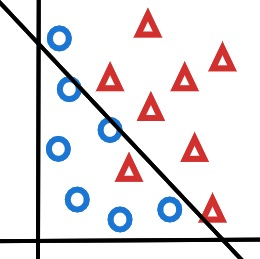
\includegraphics[width=0.4\textwidth]{MarcoTeorico/imgs/Ajuste_subajuste.jpg}
    \caption{Ejemplo de subajuste.}
    \label{fig:OverFiting}
\end{figure}


Por otro lado, tenemos un sobreajuste cuando la red modela los datos de entrenamiento demasiado bien y no se generaliza a los datos de validación (\cite{rosebrock2017deep}). En este caso tenemos que las predicciones solo serán buenas para aquellos que se utilice el mismo conjunto de datos que en el entrenamiento, Figura \ref{fig:underFiting}.

\begin{figure}[H]
    \centering
    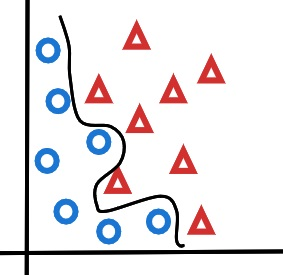
\includegraphics[width=0.4\textwidth]{MarcoTeorico/imgs/Ajuste_sobreajuste.jpg}
    \caption{Ejemplo de sobreajuste.}
    \label{fig:underFiting}
\end{figure}

Por otra parte, el entrenamiento ideal es cuando la red modela los datos de entrenamiento con cierto margen de error, pero siendo su gran mayoría correcta, Figura \ref{fig:idealFiting}.

\begin{figure}[H]
    \centering
    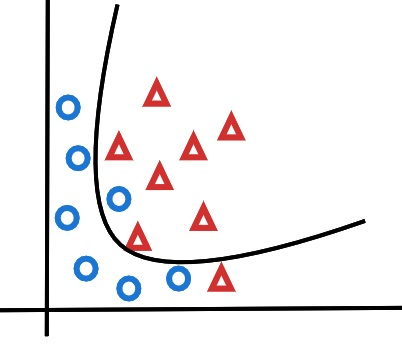
\includegraphics[width=0.6\textwidth]{MarcoTeorico/imgs/Ajuste_ideal.jpg}
    \caption{Ejemplo de ideal.}
    \label{fig:idealFiting}
\end{figure}

\subsection{Métricas de evaluación}


Ahora bien, cuando se realiza el entrenamiento es necesario saber que tan bueno es el modelo que se ha generado, para esto existen diferentes métricas que nos indican de manera cuantitativa la calidad del modelo.

Cuando se ha entrenado un modelo para un problema de clasificación se utilizan medidas de exactitud como una métrica de evaluación. La exactitud se calcula con el número de predicciones correctas entre el número de predicciones totales, La Ecuación \ref{eq:exactitud} muestra la métrica de exactitud.

\begin{equation}
    \label{eq:exactitud}
    Exactitud = \frac{Predicciones \: correctas}{ Total \: de \: predicciones}
\end{equation}

Por otra parte, los modelos creados para problemas de regresión hay tres métricas principales MAE, MSE Y RMSE.

La métrica de evaluación del Error Absoluto Medio (MAE – \textit{Mean Absolute Error} en Ingles) calcula la media de los valores absolutos de la diferencia entre los valores reales y los predichos. En otras palabras, MAE es el promedio de todos los errores sin tomar en cuenta si este error es positivo o negativo con respecto al valor real. La Ecuación \ref{eq:MAE} define el calculo de MAE.

\begin{equation}
    \label{eq:MAE}
    MAE = (\frac{1}{n}) \displaystyle\sum\limits_{i=0}^n \mid y_i - x_i \mid
\end{equation}

El Error Medio Cuadrado (MSE – \textit{Mean Square Error} en Ingles) se encarga de elevar al cuadrado el error, penalizando fuertemente los valores que se alejan demasiado del valor real esperado, con este valor se obtiene el promedio, la Ecuación \ref{eq:MSE} define el calculo de MSE.

\begin{equation}
    \label{eq:MSE}
    MSE = (\frac{1}{n}) \displaystyle\sum\limits_{i=0}^n (y_i - x_i)^{2}
\end{equation}

La Raíz del Error Cuadrático Medio (RMSE – \textit{Root Mean Square Error} en Ingles) al igual que la métrica MSE penaliza los errores altos, solo que para esta métrica se eliminan los cuadrados obteniendo la raíz del promedio obtenido con MSE. La Ecuación \ref{eq:RMSE} define el calculo de RMSE.

\begin{equation}
    \label{eq:RMSE}
    RMSE = \sqrt {
        (\frac{1}{n}) \displaystyle\sum\limits_{i=0}^n (y_i - x_i)^{2}
    }
\end{equation}
